\section{Type Predictions}
\label{sec:type_predicts}

Next I attempted to predict the type of a card.
Once again I started by predicting type based solely on 
the card name. Using the same architecture as the final
instance of my color predictor, I now predict 1 of 7 
different type categories for a card. 
The model results in 67\% accuracy. 

\subsection{Combined Input}
At this point, I started combining features to 
see if I would achieve better performance. First, 
I wanted to predict the type of a card given both
the name and the color of the card. While it wasn't
significant, the model improved by 4\% to 71\%. Predicting
the color given both the name and the type had a
similar effect of improving performance by about 3\% to
a total of 57\%. 

\begin{figure}[h!]
    \centering
    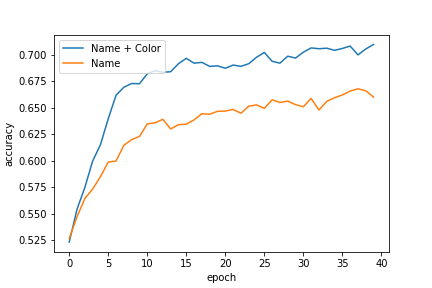
\includegraphics[width=0.9\linewidth]{figures/glove_color_vs_no.png}
    \caption{Predicting Types using Name + Color vs. Name}
    \label{fig:color_no_color}
\end{figure}
